\documentclass{mypaper}

% Nye komandoer og pakker - kk du kan bare flytte dem ind i ../mypaper
% hvis du føler for det
\newcommand\Cpp{C\raisebox{\height / 2}[\height][\depth]{\tiny ++}}
\usepackage{pdfpages} % Vi anvender \includepdf til at inkludere
                      % forsiden

\title{XY-plotter}
\author{Christian Klim Hansen \and Kristian Kjærgaard \and Nick Østergaard}
\date{\today}

\hypersetup{
  pdftitle={AceHigh, en (x,y)-plotter},
  pdfsubject={},
  pdfauthor={Christian Klim Hansen, Kristian Kjærgaard og Nick Østergaard},
  pdfcreator=LaTeX,
}

\pagestyle{Ruled}


\begin{document}

\includepdf{./img/forside}

\setcounter{page}{2}

\strut \vfill { \footnotesize
  \noindent 
  Copyright © 2009 Christian Klim Hansen, Kristian Kjærgaard og Nick Østergaard\\\\
  \noindent
  Layout af forfatterne med \LaTeX\\
  Illustrationer i Dia og Inkscape\\
  Billeder redigeret i GIMP\\
  Print diagrammer og printudlæg i KiCad
}

\thispagestyle{empty}

\clearpage

\frontmatter

\tableofcontents

\chapter{Forord}

% bl.a. tak til David Pedersen (Kjærgaards fætter) for vejledning om
% hvad? RipRap-fællesskabet (specielt fenn)

Tak til miljøet omkring den frie software. Fri tale, gratis øl og alt
det der\dots


%%% Local Variables: 
%%% mode: latex
%%% TeX-master: "../master"
%%% End: 

\mainmatter

\chapter{Indledning}

% Note om hvad der skal stå i dette afsnit her.

Følgende rapport er skrevet i forbindelse med vores afsluttende
projekt i faget El-teknik.  Vi har fået udleveret tre mulige temaer,
hvor vi har valgt at arbejde med temaet: Robotteknologi, som omfatter
følgende:

\begin{itemize}
\item Udvikling af udstyr med funktioner af robotagtig karakter
\item Dette udstyr skal virke uden menneskelig indgriben
\end{itemize}

Vi ønsker, at opfylde disse krav ved at lave en plotter, som aflæser
data fra et SD-kort. Plotteren har til formål at tegne en figur på et
stykke A4-papir \fixme{Kjærgaard:referer til kravspecifikation}. Vi
har haft i alt 100 timer pr. person fordelt ud over 10 uger. Vi har
fået stillet 300 kr. pr. person til rådighed i dette projekt til fri
benyttelse, så længde at det har en tydelig relevans for vores
projekt. Samtlige indkøb skal godkendes af læreren.


\section{Overordnede produktkrav}

Vores produkt skal indeholde følgende elementer for at overholde
produktkravene:

\begin{itemize}
\item Der skal indgå mindst et elektrisk kredsløb med passive og
  aktive komponenter udover microcontrolleren
\item Der skal designes print layout vha. CAD
\item Der skal anvendes mindst én microcontroller
\item Der skal benyttes avancerede funktioner i microcontrolleren, som f.eks.:
  \begin{itemize}
  \item Interrupt
  \item Timer
  \item Tæller
  \item U(S)ART eller ADC
  \end{itemize}
\end{itemize}


\section{Kravspecifikation}

Vi vil lave en plotter, som opfylder følgende specifikationer:

\begin{itemize}
\item Plotteren skal tegne en figur, som vi har tegnet på computer
  \begin{itemize}
  \item Skal tegne på et stykke A4-papir
  \item Fungere uden at en computer er tilsluttet
  \item Læse data fra SD-kort
  \end{itemize}
\item Kunne forstå følgende elementer af HPGL:
  \begin{itemize}
  \item Rette linier
  \item Cirkler
  \end{itemize}
\item Anvende en AVR-processor
\item Bruge en pen til at tegne
  % \begin{itemize}
  % \item Bemærk at der ikke skal benyttes blyant eller kuglepen
  % \end{itemize}
\item Styre hastigheden af pennen meget præcist
  \begin{itemize}
  \item Med software skal vi gøre optimalt nytte af stepmotorenes præcision
  \end{itemize}
\item Kunne lave nødstop og restart med knapper
  % \item Vise status af tegneforløb på LCD-display eller med lysdioder
\item Kunne gå i nulstillingsposition (et sted hvor maskinen ved den
  så er) ved tryk på en trykknap
\item Den mekaniske konstruktion skal ligne figur\vref{fig:plotterskitse}
  \mnote{
    \includegraphics[width=\marginparwidth]{img/plotterskitse}
    \captionof{figure}{Skitse af konstruktion}
    \label{fig:plotterskitse}
  }
\item Bruge tandrem til at trække x- og y-akserne
  \begin{itemize}
  \item Tandrem er forbundet med stepmotor
  \end{itemize}
\item Pennen kan løftes og sænkes
\end{itemize}


\section{Terminologi}

% Her skriver vi hvilken betydning forskellige ord har i
% rapporten. Hvad betyder fx software, MCU, plotter etc.

Med software menes den ekserkvering, der sker på mikroprocessoren i plotteren.


\section{Om kodeeksempler i rapporten}

Alt software i vores projekt er udviklet med den frie GNU AVR C
Compiler\fixme{korrektur}, som virker på både Windows og Linux.

\fixme{Terminologi og Om kodeeksempler i rapporten bør nok være i Forord}

%%% Local Variables: 
%%% mode: latex
%%% TeX-master: "../master"
%%% End: 
\chapter{Brugervejledning}
\label{ch:brugervejledning}
\mnote{Nick Østergaard}

% Interface (kanp-oversigt)
% Overførsel af data, eventuelt generering af data
% Placering af papir
% Specifikationer - tegneområde, placering af et ark papir

For at tegne grafik i HPGL-formatet, gør følgende:

\begin{enumerate}[\quad \bfseries 1.] \firmlist
\item Konverter tegningen til HPGL (hvis programmet ikke kan
  konvertere til HPGL men til PostScript, kan
  \texttt{pstoedit}\footnote{Se \url{http://www.pstoedit.net}.})
\item Brug \texttt{HPGL Distiller}\footnote{Se
    \url{http://pldaniels.com/hpgl-distiller}.} på HPGL-tegniningen.
\item Overfør tegningen til SD-kortet med
  f.eks. \texttt{dd}\footnote{Se
    \url{http://en.wikipedia.org/wiki/Dd_(Unix)}.} eller
  \texttt{HxD}\footnote{Se
    \url{http://mh-nexus.de/en/hxd}.}. SD-kortet bruger \textit{ikke}
  et filsystem, så første byte i tegningen er første byte på
  hukokmmelsesblokken.
\item Sæt SD-kortet i plotteren og flyt langsomt tegnehovedet ned i
  hjørnet.
\item Tænd for strømmen til stepmotorerne, tegnehovedet og sidst
  MCU'en. Maskinen begynder at tegne.
\end{enumerate}

\fixme{Sammen: Hvad med at angive en kort beskrivelse af dd og hxd i
  stedet for wiki link?}

%%% Local Variables: 
%%% mode: latex
%%% TeX-master: "../master"
%%% End: 

\part{Design}
\label{prt:design}

\chapter[Design af mekanik]{Mekanik}
\mnote{Nick Østergaard og Christian Klim Hansen}

% Her beskrives de overvejelser vi har haft omkring udformningen af
% vores mekanik.

I vores overvejelser omkring udformningen af vores produkt, så vi på
selve funktionen af produktet. Fordi vores produktet har til formål at
plotte en figur på et stykke A4-papir, så er det vigtigt, at
mekanikken er så slørfri som muligt. For at undgå slør har vi set på
placeringen af pennen, forskellige konstruktioner til akserne, og
hvilken metode vi vil bruge til at flytte akserne.

Vi havde to forskellige forslag til udformningen af glideren. De to
stænger, som pennen kører på, kunne enten være placeret vandret, som
ses på figur\vref{fig:glider}, eller lodret. Vi kom frem til, at det,
som ville resultere i mindst slør, var, hvis gliderne var placeret
vandret, da det giver en større stabilitet. Pennen styres af en
stepmotor, som er placeret ude i en af siderne.

\mnote{
  \includegraphics[width=\marginparwidth]{./img/glider}
  \captionof{figure}{Vandret glider}
  \label{fig:glider}
}

Et andet problem omkring slør var placeringen af stepmotoren, som skal
styre gliderne. Her kunne vi placere stepmotoren i midten af selve
konstruktionen eller ude i en af siderne. Hvis
stepmotoren blev placeret i midten af plotteren, så ville det først og
fremmest resultere i en større konstruktion, da stepmotoren skulle
placeres over glideren, men ligeledes ikke gøre meget for at hjælpe på
sløret. Hvis vi istedet placerer stepmotoren i siden, som det vises i
afsnit~\vref{sc:stepmotor-driver}, så vil den være i
samme plan som glideren, hvilket vil gøre konstruktionen en del
mindre og samtidig hjælpe på sløret. Glideren vil da først bevæge sig,
når sløret er nogenlunde væk, hvilket giver anledning til en mere
præcis plotning.

Enkelheden af konstruktionen var ligeledes en essentiel del af vores
projekt, da vi har en begrænset periode, hvori vi kan udforme vores
produkt. Produktets størrelser var dog ikke under megen diskusion, da
det simplistiske skulle være en gennemtrængende del uden at have en
indvirkning på produktets kvalitet og funktionalitet. Gliderne samt
glidelejrene er lavet i stål for reduceret gnidningsmodstand. Vi
bruger også teflonolie til yderligere at gøre modstanden mindre, og
derved mindske sløret.


%%% Local Variables: 
%%% mode: latex
%%% TeX-master: "../master"
%%% End: 
\chapter{Hardware}

% Afsnittet skal indeholdeinformation om vores
% hardware. Strømforsyning, motor drivere, MCU print, transducere m.m.

\section{Stepmotor drivere}
I dette projekt har vi to forskellige stepmotorere, som vi har fundet
fra et par bordscannere. Motorene er selvfølgelig forskellige fra
hinanden. Den ene motor er en bipolar motor mens den anden er en
variabel reluktans motor. Vi har i det følgende valgt, at lave hvert
driver print på hvert sit printkort, da vi opnår en vis fleksibilitet,
da vi på den måde lettere kan lave den ene om, i tilfælde af den anden
brænder af eller der er fejl på. \fixme{todo, Omformuler dårlige formuleringer}

\subsection{Bipolar motor}
\fixme{Nærbillede af lille motor}

\subsection{Unipolar motor}

\fixme{Husk at angive \cite{fronter:stepmotor} som kilde til dette
  afsnit på en eller anden måde} \fixme{Nærbillede af stor motor}

\section{Transducer}
Vi skal være i stand til at nulstille maskinens psition i forhold til
vores koordinat system. Til dette kunne man gøre det, at man kører
motorerne i retning med nulpunkt, men kører længere end vi kan
køre. Det sklhavetil formål, at govedet bliver trukket til norigo. Men
detdenne metode er ikke anvendelig, så dda man vil belaste mekanikken
og motorerne for meget. Derfor kan man anvende nogle transduvere. vi
kan anvende et par gaffel foto sensorer.. Vi kan så se lade maskinen
se, hvornår der kommer noget ind for sensoren, ogg i kan da stoppe
maskinen på den måde ved vi at maskinen er nulstilllet. Vi kan
harefter begynde at anvende maskinen. \fixme{nick: Dette skal
  renskrives, det er skrivet med bind for øjenene.} \fixme{nick: Der
  skal tegnes en illustration, der illustrerer placeringen af disse
  transducere}

%%% Local Variables: 
%%% mode: latex
%%% TeX-master: "../master"
%%% End: 
\chapter[Design af software]{Software}

% Note om hvad der skal stå i dette afsnit her.


\section[Motorstyring]{Motorstyring\footnote{Se rettelser til dette
    afsnit i afsnit\vref{ssc:rettelse-design}.}}

\mnote{Kristian Kjærgaard}

Dette afsnit diskuterer forskellige metoder til at styre tegnehovedets
placering.

Hastigheden for tegnehovedet er givet ved
\begin{align}
  v = \frac{\Delta x}{\Delta t} \label{eq:hastighed}
\end{align}
hvor $v$ er hastigheden, $\Delta x$ er positionsændring og $\Delta t$ er
tidsændring. En præcis styring af hastighed kræver et præcist kendskab
til både positionsændring og tidsændring.

Den mindst mulige positionsændring er ét step med stepmotoren og
kendskabet til denne er tilstrækkeligt.

Følgende to afsnit diskuterer to forskellige metoder til at
\textit{time} motorerne.


\subsection{Motorstyring med indlagt forsinkelse}

En metode at styre timingen på er ved at afvikle tidsberegningen på en
tråd med indlagt forsinkelse, således at vi beregner den tid $\Delta t
= \frac{\Delta x}{v}$, vi skal vente, se
figur\vref{fig:motorstyring-indlagt-forsinkelse}.

\begin{figure}[htbp]
  \centering
  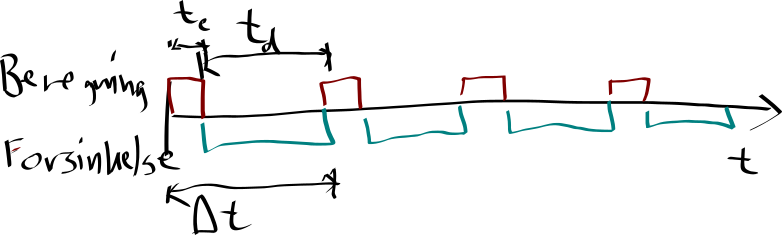
\includegraphics[width=.5\textwidth]{./img/motorstyring-indlagt-forsinkelse}
  \caption{Motorstyring med indlagt forsinkelse.}
  \label{fig:motorstyring-indlagt-forsinkelse}
\end{figure}


For denne metode gælder, at tidsændringen $\Delta t$ er summen af den
tid, det tager af afvikle beregningen $\frac{\Delta x}v$ og den tid,
der indlægges som forsinkelse:
\begin{align}
  \Delta t &= t_e + t_d \Rightarrow \label{eq:afbrudt-afvikling-tid} \\
  v &= \frac{\Delta x}{t_e + t_d}
\end{align}
hvor $t_d$ er den indlagte forsinkelse, og $t_e$ er den tid det tager
at afvikle tidsberegningen (se figur\vref{fig:motorstyring-indlagt-forsinkelse}).

Ekserkveringstiden $t_e$ kan variere og kendes ikke på
afviklingstidspunktet. Derfor er metoden upræcis -- specielt ved høje
hastigheder. Figur\vref{fig:motorstyring-indlagt-forsinkelse-timing}
viser, hvordan $t_e$ får større indflydelse på $\Delta t$ ved høje
hastigheder.

\begin{figure}[htbp]
  \centering
  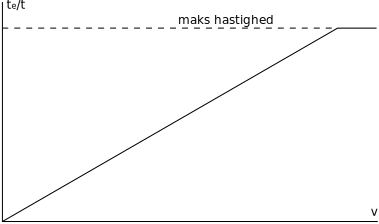
\includegraphics[width=.8\textwidth]{./img/tid-hastighed-forhold-indlagt-forsinkelse.pdf}
  \caption{Hastighed som funktion af forsinkelse for motorstyring med
    indlagt forsinkelse.}
  \label{fig:motorstyring-indlagt-forsinkelse-timing}
\end{figure}

Softwaren designes \textit{ikke} på denne måde.


\subsection{Motorstyring med afbrudt afvikling}

Alternativt kan motorerne times med afbrudt afvikling. Tiden går mens
det beregnes til hvilket tidspunkter, motorerne skal køres frem til
næste step. Når vi når til et sådant tidspunkt, afbrydes afviklingen
af tidsberegningen, mens motorerne flyttes. Når motorerne er flyttet,
genoptages afviklingen af tidsberegningen, se
figur\vref{fig:motorstyring-afbrudt-afvikling}.

\begin{figure}[htbp]
  \centering
  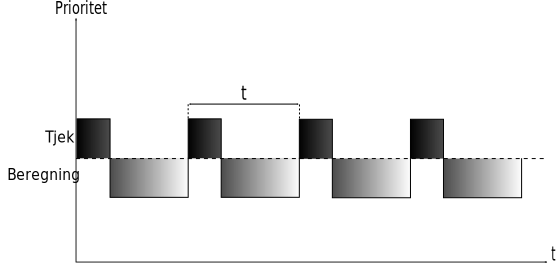
\includegraphics[width=.8\textwidth]{../brugere/kjaergaard/motorstyring-afbrudt-afvikling}
  \caption{Motorstyring med afbrudt afvikling.}
  \label{fig:motorstyring-afbrudt-afvikling}
\end{figure}

Den algoritme, der beregner næste tidspunkt, motorerne skal flyttes
på, afvikles hele tiden. Når det er tid til at tjekke, om vi har
overskredet et tidspunkt, afbrydes afviklingen af tidsberegningen,
mens motorerne flyttes. Bagefter fortsættes afviklingen af
tidsberegningen. \fixme{Kjærgaard: Er det ikke det der står ovenover?}

Denne løsning udmærker sig ved at graden af præcis styring af
hastigheden ikke afhænger af hastigheden selv, så længe afviklingen
kan foretages inden en \textit{deadline} nåes.

Løsningen forudsætter, at
\begin{itemize} \firmlist
\item der periodisk tjekkes, om vi har overskredet et tidspunkt,
\item dataene fra algoritmen, der beregner tidspunkter, kan opbevares
  i en kø (først-ind-først-ud struktur, bruges ofte som
  \textit{buffer}),
\item der er data i køen, når det tjekkes, om vi har overskredet et
  tidspunkt, og
\item tidsberegningen kan afvikles så hurtigt, at der lægges data i
  køen hurtigere end der periodisk tjekkes for data.
\end{itemize}

Softwaren designet med afbrudt afvikling.


\subsection{Algoritme til tidsberegning}

\mnote{Christian Klim Hansen}

Forholdet imellem tiden det tager at tegne linjen og tiden til et
punkt $x$ på linjen er lig forholdet imellem det givne punkts $x$-koordinat
og forskellen imellem start- og slutkoordinat $\Delta x$:
\begin{align}
  \frac{t}{\Delta t} &= \frac{x}{\Delta x} \qquad \Rightarrow \nonumber \\
  x &= \Delta x \times \frac{t}{\Delta t} \label{eq:x-af-dxtdt}
\end{align}

Her forudsættes det, at hele linjen tegnes med konstant hastighed. Se
figur\vref{fig:matematik-skitse} for geometrisk fremstilling.

\mnote{
  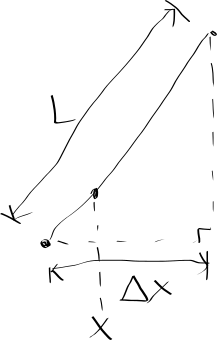
\includegraphics[width=\marginparwidth]{./img/matematik-skitse}
  \captionof{figure}{En skrå linie med positionsændring $\Delta x$
    angivet for $x$-aksen}
  \label{fig:matematik-skitse}
}


Den tid $\Delta t$ det tager at tegne linjen, er givet ved:
\begin{align}
\Delta t = \frac Lv \label{eq:v-af-lv}
\end{align}

Vi kombinerer \eqref{eq:x-af-dxtdt} og \eqref{eq:v-af-lv} og isolerer
$t$:
\begin{align}
t \times \frac{x}\Delta x &= \frac Lv \Leftrightarrow \\
t &= \frac{x}\Delta x \times \frac Lv \label{eq:t-af-dxxlv}
\end{align}

Længden af linjen $L$ er givet ved ud fra pythagoras læresætning:
\begin{align}
L &= \sqrt{\left(\Delta x\right)^2 + \left(\Delta y\right)^2}
\end{align}

Forholdet imellem positionen $x$ og positionsændring $\Delta x$ er lig
forholdet mellem step $n_x$ og stepændring $\Delta n_x$:
\begin{align}
\frac{x}{\Delta x} = \frac{n_x}{\Delta n_x} \label{eq:xdx-af-nxdnx}
\end{align}

Sætning \eqref{eq:t-af-dxxlv} og \eqref{eq:xdx-af-nxdnx} kombineres
til udtrykket:
\begin{align}
t &= \frac{n_x}{\Delta n_x} \times \frac{L}{v} \label{eq:t-af-nxdnxlv}
\end{align}

Opløsningen for $x$-retningen er givet ved:
\begin{align}
  n_x = x \times \eta_x \label{eq:eta}
\end{align}

Alle symboler med indeks $x$ gælder kun for $x$-aksen. Der arbejdes
med tilsvarende symboler med indeks $y$ for $y$-aksen.


\section{HPGL -- Hewlett-Packard Graphics Language}
\label{sec:hpgl}
\fixme{Kjærgaard: Skal det hedde dataformat i stedet?}

Når man skal vælge, hvilket dataformat man vil bruge, når man laver en
plotter, så er det vigtigt at se på fordele og ulemper se tabel
\vref{tbl: fordele og ulemper ved eget dataformat} og
\vref{tbl: fordele og ulemper ved hpgl}. Der findes mange
forskellige standarder, som kan anvendes, og en af disse standarder er
HPGL, som vi benytter os af.

\begin{table}[htbp]
  \centering
  \caption{Fordele og ulemper ved eget dataformat}
  \begin{tabular}{p{5cm} p{5cm}}
    \toprule
    % vil gerne have \centering på de to overskrifter men kan ikke
    % finde ud af det
    \bfseries Fordele & \bfseries Ulemper \\
    \midrule
    { \begin{itemize} \firmlist
      \item Vi kan gøre det så simpelt som muligt, både til at læse og
        til at forstå
      \end{itemize} }
    &
    { \begin{itemize} \firmlist
      \item Det vil nok afføde børnesygdomme
      \item Der findes ikke software, som kan håndtere vores
        dataformat
      \end{itemize} } \\
    \bottomrule
  \end{tabular}
\label{tbl: fordele og ulemper ved eget dataformat}
\end{table}
\fixme{Fix layout på tabel (punktform?)}

Vi kunne i princippet godt udvikle vores eget
dataformat, men dette vil både være meget tidskrævende, og
samtidigt vil det være svært at få implementeret, da vores format ikke
ville være en standard, og derfor ville der ikke være noget som direkte virkede med
det. Derimod er HPGL velegnet i vores projekt, da det er mere
virkelighedsnært at benytte en standard, som allerede er konstrueret
som et plotterformat, samtidig med at det kan anvendes af forskellige
applikationer (andre CAD programmer). Der er heller ikke mange ulemper
tilknyttet til brugen af HPGL som plotterformat. Det vil dog tage lang
tid at implementere det hele, hvilket vi dog heller ikke gør. Vi
kommer f.eks. ikke til at benytte os af pin-skrift og en del andre
ting, men disse problemer er relativt lette at komme udenom. Figur
\vref{tab:hpgl-fordele-ulemper} viser vores overvejelser om brugen
af HPGL som dataformat.

%Når man betragter HPGL som et plotterformat, så betyder det, at den
%indeholder mange forskellige kommandoer med hver deres funktion. Det
%kan tage lang tid at sætte sig ind i alle disse ting, men hvis man har
%forståelse for, hvilke funktioner vi evt. kommer til at bruge i vores
%projekt, vil det selvfølgelig lette indlæringsarbejdet en del.

%Følgende er en tabel over vores overvejelser omkring fordele og
%ulemper ved brugen af eget dataformat samt fordele og ulemper ved
%brugen af HPGL:

%Dette betyder, at der findes ingen software, der kan håndtere
%formatet. Dette betyder at vi selv skal skrive den software, som er
%uden for rammer af dette projekt. Derfor leder vi efter en
%eksisterende standard.


\begin{table}[htbp]
  \centering
  \caption{Fordele og ulemper ved HPGL.}
  \label{tab:hpgl-fordele-ulemper}

  \begin{tabular}{p{5cm} p{5cm}}
    \toprule
    Fordele & Ulemper \\
    \midrule
    { \begin{itemize} \firmlist
      \item Afprøvet og bruges industrielt til plottere
  	  \item Veldokumenteret
      \item Der findes software, som kan håndtere HPGL
      \end{itemize} }
    &
    { \begin{itemize} \firmlist
      \item Niveauet er sat højt, hvilket betyder, at der er mange
        funktioner som vi ikke får brug for
      \item Implementeringstiden er længere
      \end{itemize} }
    \\
    \bottomrule
  \end{tabular}
\label{tbl: fordele og ulemper ved hpgl}
\end{table}


Dette betyder, at HPGL er meget velegnet til brug i vores projekt, da
formatet er veldokumenteret, afprøvet og anvendt industrielt til
specielt plottere, hvilket vores eget selvfølgelig også ville være. Samtidig
finde allerede software, som kan håndtere formatet til forskel fra
vores eget. Implementeringstiden vil dog være en del længere, da
niveauet er sat fra starten, hvilket medfører en del ubenyttede
funktioner.


\section{Koordinatsystem}
\mnote{Kristian Kjærgaard}

% Skriv om koordinatsystemet

Vi arbejder med skærmkoordinater (se
figur\vref{fig:skaermkoord}). HPGL (se afsnit\vref{sec:hpgl}) er
formateret i skærmkoordinater (Cartesiansk koordinatsystem med én
kvadrant, $x$-akse voksende mod højre og $y$-akse
voksende ned), og internt i softwaren kan en konvertering springes
over ved at bruge skærmkoordinater.

\mnote{
  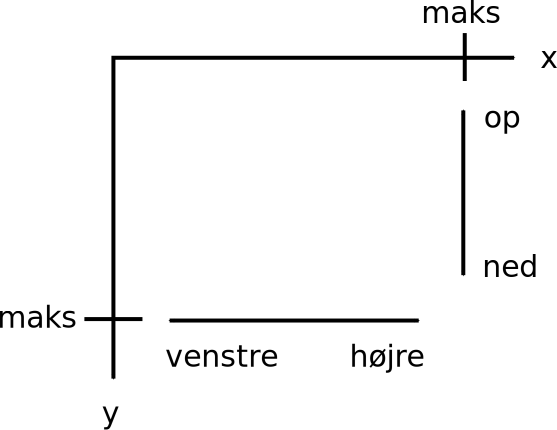
\includegraphics[width=\marginparwidth]{../brugere/kjaergaard/skaermkoordinater}
  \captionof{figure}{Skærm\-koor\-dinater. Der arbejdes med
    skærm\-koordinater i plotteren.}
  \label{fig:skaermkoord}
}

\section[Valg af programmeringssprog]{Valg af
  programmeringssprog\footnote{Se rettelser til dette afsnit i afsnit\vref{sec:bilag-programmeringssprog}}}
\fixme{henvisning}

Softwaren skrives i C og \Cpp.

C bruges i moduler, hvor sproget uden videre er tilstrækkeligt. Dette
vil typisk være lavniveaumoduler, og her er C fordelagtigt, fordi det
giver større kontrol.

\Cpp\ bruges i moduler, hvor det er fordelagtigt at bruge
\Cpp-speficikke elementer (f.eks. generisk programmering\fixme{note om
  dette?}). Moduler, der afhænger af moduler skrevet i \Cpp, vil
typisk også være skrevet i \Cpp.

Alle C-moduler er kompatible med \Cpp, og alle \Cpp-moduler er så vidt
muligt kompatible med C. Uønskede sideeffekter af \Cpp\ forsøges
undgået (\fixme{eksempler her!}). \Cpp\ bruges ikke objektorienteret.



%%% Local Variables: 
%%% mode: latex
%%% TeX-master: "../master"
%%% End:

\part{Implementering}
\label{prt:implementering}

\chapter[Implementering af mekanik]{Mekanik}
\mnote{Nick Østergaard}

% Note om hvad der skal stå i dette afsnit her.
% Kort afsnit om hvordan vi har lavet vores produkt ud fra vores
% overvejelser

Figur \fixme{Indsæt figur over færdigt produkt} viser vores færdige
produkt.  Udformningen af produktet tager udgangspunkt i vores
overvejelser i design-afsnittet.  Man ser ud fra figuren, at akserne
styres af to stepmotor, som er henholdsvis uni- og bipolar.  Vi
startede med at lave basen for vores produkt. Her tog vi udgangspunkt
i, at vi skulle kunne tegne på et stykke A4-papir. Yderligere havde vi
brug for plads til vores hardware, som styrer stepmotorerne. Herefter
blev gliderne og deres respektive dele lavet og sat sammen med basen,
som det fremgår af figuren. Vi havde brug for en holder til pennen,
som passede med gliderne, så det var naturligt at lave denne i den
afsluttende del af produktionsforløbet.

\section{Tegnehovedet}\fixme{Under mekansik}
Tegnehoved er i afsnittet\vref{sc:d-tegnehoved} beskrevet som en
penholder. Vores tegnehoved er konstrueret som det ses på
figur\vref{fig:tegnehoved-skitse}.

På en glider, er der monteret en trækmagnet, som er forbundet mekanisk
til en arm der holder pennen. Armen holdes oppe af en fjeder. Når man
aktiverer trækmagneten, vil

\begin{figure}[htbp]
  \centering
  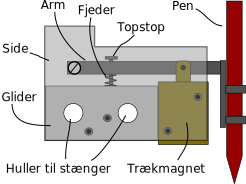
\includegraphics[width=7cm]{./img/tegnehoved-skitse}
  \caption{Skitse af tegnehoved}
  \label{fig:tegnehoved-skitse}
\end{figure}

\mnote{
  \includegraphics[width=\marginparwidth]{./img/tegnehoved}
  \captionof{figure}{Tegne\-hovedet i dets reele form}
  \label{fig:tegnehoved}
}

%%% Local Variables: 
%%% mode: latex
%%% TeX-master: "../master"
%%% End: 
\chapter[Implementering af hardware]{Hardware}
\mnote{Nick Østergaard}

% Vi skriver her om hvordan vi faktisk realiserer det vi har sankket
% om i Hardwaredesignet

\section{Stepmotor driver}
\label{sc:stepmotor-driver}
\fixme{Omformuleres!}Vi skal konstruere en
stepmotor driver med et par integrerede stepmotor drivere. Mere
specefikt anvender vi et par L6208N'ere, som kan styre en bipolar
stepmotor. Vi bruger denne driver, da den er simpel at styre, samt der
er mulighed for at lave strømbegrænsning. Hvilket vil gøre, at vi kan
skrue forsyningsspændingen til motorerne op og begrænse strømmen,
således motorerne er mere kvik, hvilket betyder at vi kan køre
hurtigere.


\mnote{
  \includegraphics[width=\marginparwidth]{./img/stepmotordriver}
  \captionof{figure}{Stepmotor driver}
  \label{fig:stepdriver}
}
\fixme{Nick: Beskær billede}

\mnote{
  \includegraphics[width=\marginparwidth]{./img/x-motor}
  \captionof{figure}{X-aksens motor monteret}
  \label{fig:x-motorimg}
}

\mnote{
  \includegraphics[width=\marginparwidth]{./img/y-motor}
  \captionof{figure}{Y-aksens motor monteret}
  \label{fig:y-motorimg}
}

\section{Sensorerne}
\fixme{delkredskøb til gaffelsensorerne}

\mnote{
  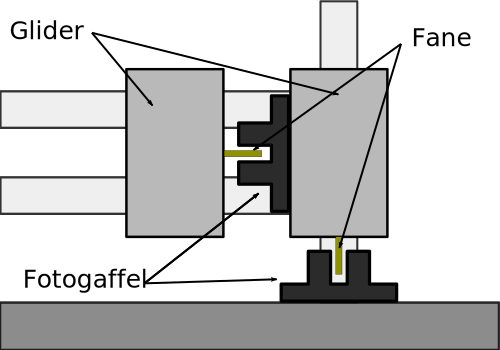
\includegraphics[width=\marginparwidth]{./img/fotogafel-skitse}
  \captionof{figure}{Placering af fotogafler}
  \label{fig:transducer-skitse}
}
\fixme{nick: Illustrationen af sensorerne skal laves rigtigt}

\mnote{
  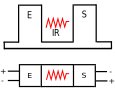
\includegraphics[width=\marginparwidth]{./img/fotogaffel}
  \captionof{figure}{Skitse af fotogaffel}
  \label{fig:fotogaffel-skitse}
}

\section{SD-kort adapter}
Som følge af at vi har bestemt i vores kravspecifikation, at vi skal kunne lægge data på et
SD-kort, og få poltteren til at tegne det vi har bestemt i dataene, så
skal vi selvfølgelig også have lavet en SD-kort adapter.

Vi har ved at kigge på litteratur \cite{web:captain-mmc} og
\cite{web:sd-pinout}, konstrueret en SD-kort adapter vi kan bruge til
vores ATmega128 print.

\fixme{Billede af SD-kort adapter}
\fixme{Printlayout og pinout}

\fixme{Beskriv kort, hvordan vi aktiverer vores sænker}

%%% Local Variables: 
%%% mode: latex
%%% TeX-master: "../master"
%%% End: 

\chapter[Implementering af software]{Software}

% Note om hvad der skal stå i dette afsnit her.


\section{Oversigt over softwaren}

% Her skriver vi hvordan softwaren er struktureret - se figuren nedenfor.

Softwaren er struktureret som vist i
figur\vref{fig:software-oversigt}. Dataføderen leverer data til den
del af softwaren, der behandler HPGL. Dataen kommer fra et
SD-kort. HPGL-behandleren sender instruktioner videre til den del af
motorkontrollen, der afvikles når der er tid. Denne del sætter
instruktioner i kø til realtidsdelen.

Realtidsdelen af motorkontrollen behandler de instruktioner, den anden
del af motorkontrollen har sat i kø og styrer stepmotorer m.m. efter
disse instruktioner. Realtidsdelen af motorkontrollen har ansvar for,
at hastigheden af tegnehovedet kan styres præcist.


\begin{figure}[htbp]
  \centering
  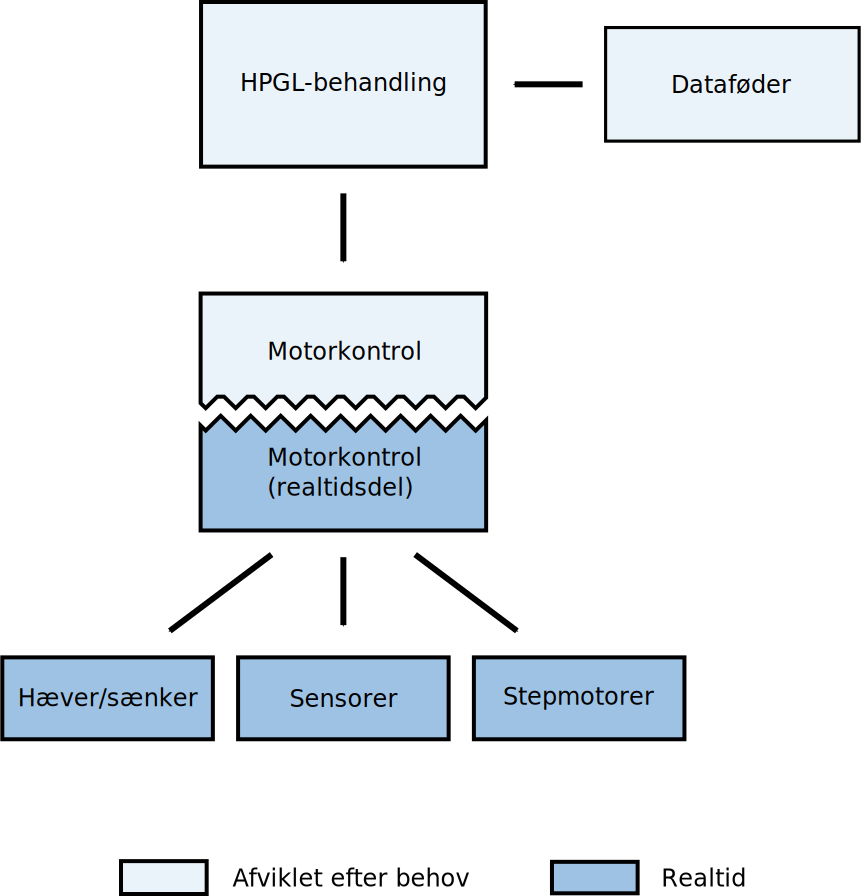
\includegraphics[width=.75\textwidth]{../brugere/kjaergaard/software-oversigt}
  \caption{Oversigt over softwaren. De lyseblå dele afvikles når der
    er tid til det. Når det er tid til at afvikle de mørkeblå områder,
    afbrydes afviklingen af de lyseblå.}
  \label{fig:software-oversigt}
\end{figure}


\section[Dataføder (med SPI og SD-/MMC-kort)]{Dataføder}

% Hvordan virker dataføderen (herunder buffer, spi og sd/mmc)?

Dataføderen leverer data til HPGL-motoren og håndterer de
underliggende moduler, der indeholder data.

Dataføderens skal
\begin{itemize} \firmlist
\item levere data til HPGL-motoren og sørge for at denne ikke løber
  tør for data\fixme{bliv enig om terminologi}
\item stille et uniformt API\footnote{Application Programming
    Interface, programmeringsbrugerflade; betegnelse for struktur og
    navngivning for funktioner, variable, strukturer, klasser
    etc. brugt til programudvikling.}\fixme{brug evt. wikis
    formulering af api} til rådighed uafhængig af underliggende modul,
  således at det overliggende modul er uafhængig af det modul, der
  indeholder data - se figur\vref{fig:datafeeder-uniform-api}
\item håndtere fejl for underliggende moduler
\end{itemize}

\mnote{
  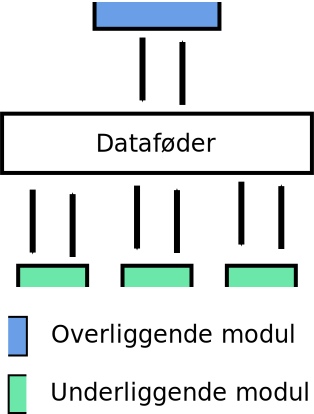
\includegraphics[width=\marginparwidth]{../brugere/kjaergaard/datafoeder-uniform-api}
  \captionof{figure}{Data\-føderen skal stille et uniformt API til
    rådighed.}
  \label{fig:datafeeder-uniform-api}
}

En oversigt over funktionsfordelingen\fixme{andet ordvalg} i
dataføreren\fixme{andet ordvalg} kan ses i
figur\vref{fig:software-spi-sd-oversigt}.

\begin{figure}[htbp]
  \centering
  \includegraphics[width=\textwidth]{../brugere/kjaergaard/datafeeder-oversigt}
  \caption{Diagram over funktionsfordeling i dataføderen.}
  \label{fig:software-spi-sd-oversigt}
\end{figure}

Kommunikationen med SD-kortet foregår gennem SPI'en.\fixme{afsnit skal
  skrives færdig}. En eksempel på en forespørgsel med tilhørende svar
kan ses i figur\vref{fig:software-spi-sd-handling}.

\begin{figure}[htbp]
  \centering
  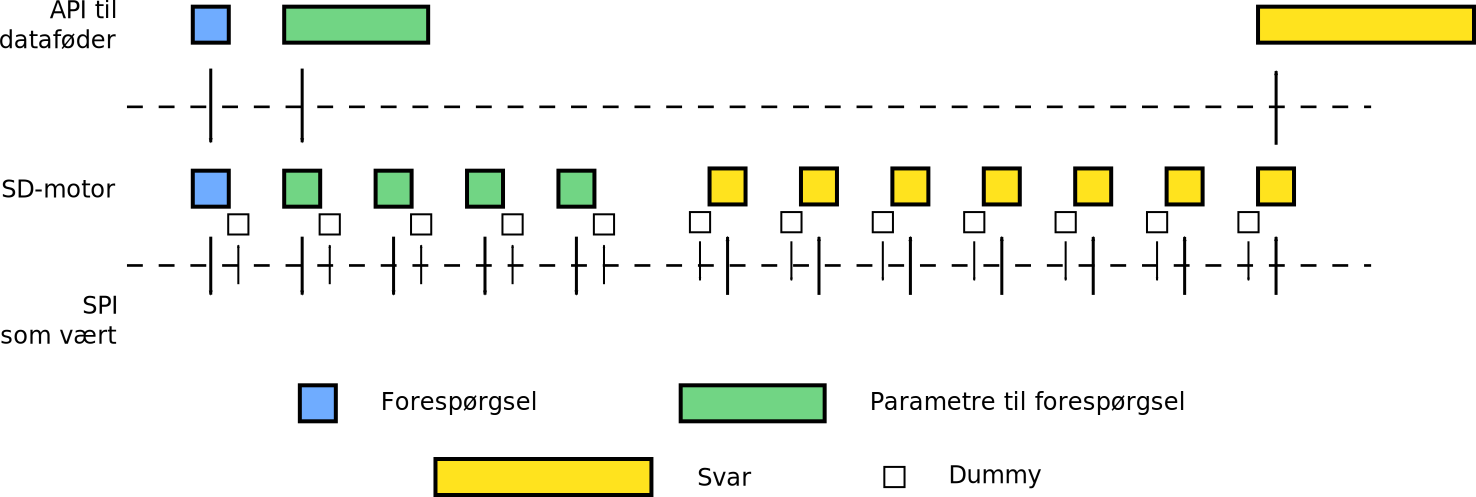
\includegraphics[width=\textwidth]{../brugere/kjaergaard/datafeeder-handling}
  \caption{Handlingdiagram ved kommunikation med SD-kortet.}
  \label{fig:software-spi-sd-handling}
\end{figure}


\section{HPGL-behandleren}

% Hvordan virker den del, der fortolker og behandler HPGL?


\subsection{Identifikation af instruktioner og parametre}

% Her skriver vi hvordan vi identificerer instruktioner og parametre i
% datastrømmen



\subsection{Matematik -- Cirkel}
\mnote{
  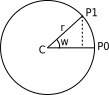
\includegraphics[width=\marginparwidth]{./img/Cirkel}
  \captionof{figure}{Cirkel}
  \label{fig:cirkel-tegning}
}
Vi kender cirklens radius, kordevinklen samt startkoordinater. Det første koordinat kan derfor let findes:
\begin{align*}
P_0(x, y)=(r, 0)
\end{align*}

Næste koordinat ligger i en vinkel v, som svarer til kordevinklen c. Ved brug af cosinus og sinus samt radius kan vi bestemme det næste koordinat:
\begin{align*}
P_1(x, y)&=(\cos(v)\times r, \sin(v)\times r)\Rightarrow \\
P_1(x, y)&=(\cos(c)\times r, \sin(c)\times r)
\end{align*}
 
Denne formel kan omskrives, så den gælder et vilkårligt punkt på cirkelperiferien:
\begin{align}
P_n(x, y)=(\cos(n\times c)\times r, \sin(n\times c)\times r)
\end{align}

Vi betragter nu en cirkel med en radius på 5cm og en kordevinkel på $3\degree$. Første koordinat er således:
\begin{align*}
P_0(x, y)=(\cos(0\times 3\degree , \sin(0\times 3\degree)\times 5)=(5, 0)
\end{align*}

Vi ser, at dette passer i overensstemmelse med første udsagn. Vha. ovenstående formel kan vi blot lægge en til n hver gang funktionen er udført. Dette skal den blive ved med indtil vinkel overskrider $360\degree$.


Der opstår dog et problem, hvis vinklen ikke går op i $360\degree$, såsom vinklen $7\degree$. $51\times 7\degree = 357\degree \Rightarrow rest = 3\degree$. Overskrider vinklen de $360\degree$, har vi to muligheder:
\begin{itemize} \firmlist
\item Funktionen afsluttes uden at slutte cirklen
\item Funktionen ændres, så optegningen fortsætter til udgangspunktet $P_0$
\end{itemize}
Det skal også nævnes, at HPGL tegner uanset om pennen er oppe eller nede, hvilket betyder, at vi skal bruge en funktion til at hæve og sænke pennen. Pennen starter i cirklens centrum. Vi skal derfor sikre os, at pennen er hævet før den går til første punkt  . Herefter bruger vi den generelle funktion til at bestemme x,y-koordinaterne. Efter hver udført funktion lægges en ekstra kordevinkel til vinklen indtil vinklen v er større eller lig $360\degree$. Herefter hæves pennen og flyttes tilbage til cirklens centrum. Afviklingsdiagrammet viser denne proces (se \vref{fig:hpgl-cirkel-afvikling}).

\begin{figure}[htbp]
  \centering
  \includegraphics[width=0.5\textwidth]{./img/Afviklingsdiagram_Cirkel}
  \caption{Afviklingsdiagram for cirkelplot}
  \label{fig:hpgl-cirkel-afvikling}
\end{figure}

\section[Motorkontrol (med buffer)]{Motorkontrol}

% Hvordan er motorkontrollen implementeret? Beskriv implementeringen
% kort.


\section{Stepmotorstyring}

% Hvordan styres stepmotorerne? Superkort. Hvordan ser softwaren der
% styrer dem ud?


\section{Sensorer og løfter/sænker}


\section{HPGL -- Hewlett-Packard Graphics Language}

% Hvordan implementerer vi HPGL? Hvilke afvigelser tillader vi os at
% tage fra den dokumentation, vi har fundet?


%%% Local Variables: 
%%% mode: latex
%%% TeX-master: "../master"
%%% End: 

\backmatter

\chapter{Afslutning}
\label{ch:afslutning}

% Fik vi opfyldt de overordnede produktkrav og vores egen
% kravspecifikation? Kom produktet til at virke? Hvis ikke hvad så? Og
% ellers som vi plejer med en konklusion...

% Vis billede af tux og logo

\section{Delvis men dækkende implementering af HPGL}

Instruktionerne \texttt{PU}, \texttt{PD}, \texttt{PA}, \texttt{PR} og
\texttt{CI} er implementeret, og det er kun en lille del af hele
HPGL-formatet. Dog viser det sig tilsyneladende, at
\texttt{pstoedit}\footnote{Se brugervejledningen
  side~\pageref{ch:brugervejledning}.} kun bruger instruktionerne
\texttt{PU}, \texttt{PD} og \texttt{PA}, så implementeringen er
dækkende til tegninger genereret af \texttt{pstoedit}.


\section{Kvalitet af plottet}

I figur\vref{fig:plot-tux} ses Tux -- Linux-maskotten -- som
vektorgrafik og som plot i plotteren. Vektorbilledet er brugt til at
generere HPGL-billedet brugt til plottet.


\begin{figure}[htbp]
  \centering
  \subfloat[Billede af Tux, fra \cite{bbt:tux-billede}.]{
    
\includegraphics[width=0.40\textwidth]{./img/Tux-simple}
  }
  \qquad
  \subfloat[Plot af billede.]{
    \includegraphics[width=0.40\textwidth]{./img/tux-plot}
  }
  \caption{Demonstration af kvaliteten af et plot.}
  \label{fig:plot-tux}
\end{figure}

\fixme{ALLE! Sørg for at vi har fået angivet skribent(er) ved alle afsnit}

%%% Local Variables: 
%%% mode: latex
%%% TeX-master: "../master"
%%% End: 


\part{Bilag}
\appendix

\chapter{Rettelser i softwaredesign og -implementering}

% Vi havde problemer med vores software - her skriver vi hvordan vi
% ende med at designe og implementere vores software

Grundet tekniske problemer er softwaren designet og implementeret
anderledes end tidligere beskrevet. Dette afsnit beskriver forskellen.

\section{Rettelser i softwaredesign}

\subsection{Valg af programmeringssprog}
\label{sec:bilag-programmeringssprog}

Grundet tekniske problemer er al softwaren skrevet i C. Desuden
unødvendiggjorde det egentlige design nødvendigheden af særlige
egenskaber ved \Cpp .

\section{Rettelser i softwareimplementering}


%%% Local Variables: 
%%% mode: latex
%%% TeX-master: "../master"
%%% End: 

\chapter{SD-kort-adapter}
\label{ch:b-sd}
\mnote{Nick Østergaard}

\begin{figure}[htbp]
  \centering
  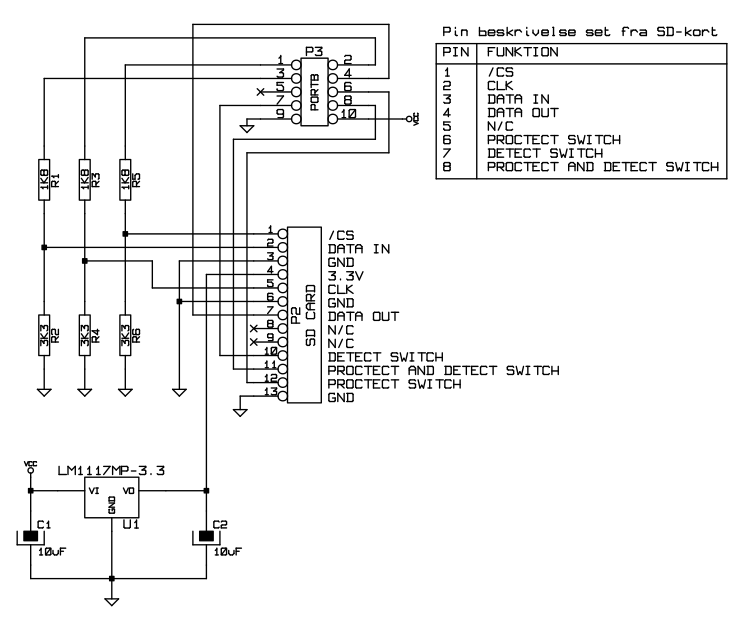
\includegraphics[width=\textwidth]{./img/sd-kort-adapter-diagram}
  \caption{Kredsløbsdiagram over SD-kort-adapteren}
  \label{fig:label-her}
\end{figure}

\mnote{
  \includegraphics[width=\marginparwidth]{./img/sdcard_9p}
  \captionof{figure}{SD-kortets benforbindelser}
  \label{fig:sdpinout}
}

\begin{figure}[htbp]
  \centering
  \includegraphics{./img/sd-kort-adapter-kobber}
  \caption{Printudlæg af SD-kort-adapteren}
  \label{fig:label-her}
\end{figure}

\chapter{L6208N driver}
\label{b-l6208n}
\mnote{Nick Østergaard}

\begin{figure}[htbp]
  \centering
  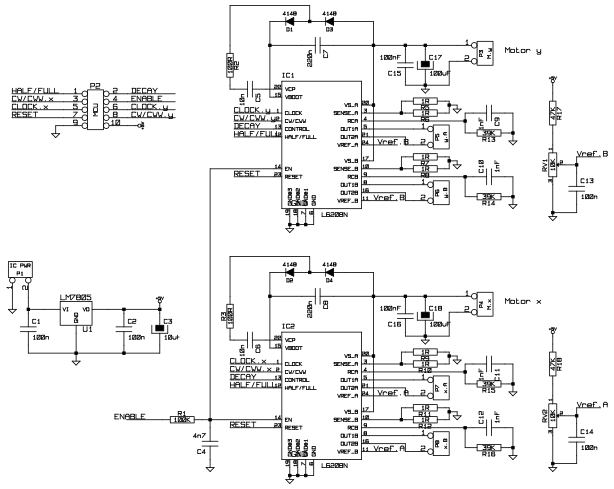
\includegraphics[width=\textwidth]{./img/l6208n-driver-diagram}
  \caption{Kredsløbsdiagram over L6208N bipolar stepmotordriveren}
  \label{fig:l6208n-diagram}
\end{figure}

\begin{figure}[htbp]
  \centering
  \includegraphics{./img/l6208n-kobber}
  \caption{Printudlæg af for vores L6208N stepmotordriver}
  \label{fig:l6208n-print}
\end{figure}

\nocite{*}
\bibliographystyle{plain}
\bibliography{litteratur}
\label{ch:litteratur}

\listoffigures

\listoftables

\listoffixmes

\end{document}
